\part{Pontuação}

\begin{table}[h]
		\centering
		\caption{Ganho de pontos}
	\begin{center}
	\begin{tabular}{|l|l|}
		\hline
			Pontos & Critérios \\ % Note a separação de col. e a quebra de linhas
	
		\hline                               % para uma linha horizontal
			(100*Nível atual) pontos & Nível completo \\
		\hline	10 pontos & Coletar estrela \\
		\hline	15 pontos & Coletar cubo \\
		\hline	20 pontos & Coletar bola \\
		\hline
 
	\end{tabular}
	\end{center}
\end{table}

\begin{figure}[!h]
	\centering
	\subfloat[Estrela]{
		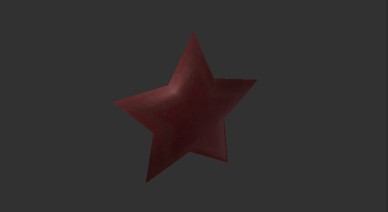
\includegraphics[height=3.5cm]{figuras/estrela}
	}
	\quad
	\subfloat[Cubo]{
		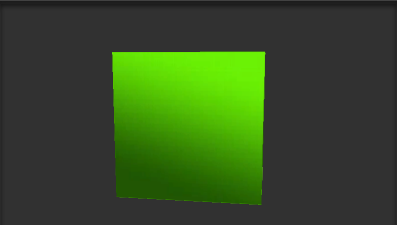
\includegraphics[height=3.5cm]{figuras/cubo}
	}
	\quad
	\subfloat[Bola]{
		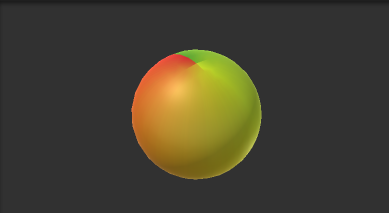
\includegraphics[height=3.5cm]{figuras/bola}
	}
	\caption{Objetos para pontuação}
\end{figure}

\begin{table}[h]
		\centering
		\caption{Perda do jogo}
	\begin{center}
	\begin{tabular}{|l|l|}
		\hline
			Pontos & Critérios \\ % Note a separação de col. e a quebra de linhas
	
		\hline Fim da corrida & Sair da pista \\
		\hline
 
	\end{tabular}
	\end{center}
\end{table}